\documentclass{article}

\usepackage{fontspec}%unicode font support

\usepackage{graphicx}%for pictures

\usepackage{geometry}%define the size of the page
\geometry{paperwidth=85mm, paperheight=55mm, layoutwidth=85mm, layoutheight=55mm, left=0mm, top=0mm, right=0mm, bottom=0mm}

\usepackage{xcolor}%setup colors
\definecolor{bl}{RGB}{0,62,92}

\usepackage[absolute,%showboxes %uncomment showboxes to see the boxes of text
verbose,overlay]{textpos}%the package for precise positioning of the text
\usepackage{tikz}%if we want to use millimeter grid
\setmainfont[Numbers={OldStyle,Monospaced}]{EB Garamond}

\pagestyle{empty}%remove all inherited formatting for the page
 
\newcommand{\phonei}{T. +33~(0)1~69~33~49~30 - M.  +33~(0)6~50~83~65~50}%+33169334930 

\newcommand{\emailii}{timofey.zakrevskiy@polytechnique.edu}
\newcommand{\urli}{www.centremaths.polytechnique.fr}
\begin{document}%
\begin{textblock*}{50mm}[0,0](4.2mm,4.2mm)%
\noindent%

\includegraphics[height=20.6mm]{LogohorEPS.eps}%
\end{textblock*}%[0,0] means that we are positioning the upper left corner of the block. (x,y) are the coordinates
 %
\begin{textblock*}{20mm}[1,0](80.2mm,4.2mm)% comment this whole block if you don't want to use the second logo
\noindent%

\includegraphics[height=20mm]{LogoCMLSTZ.png}% replace LogoCMLSTZ.png by the name of your file if you intend to use your own logo.
\end{textblock*}% [1,0] - upper right corner
%ø
\setmainfont{EB Garamond}%
\fontsize{12}{14.4}\selectfont% \fontsize{x}{y} : x Fontsize, y - interline interval
\begin{textblock*}{65mm}[0,0](18.5mm,24.8mm){\color{bl}\noindent Timofey Zakrevskiy\\*%
\setmainfont{EB Garamond}%selecting font. Put whatever you want here. This font resembles the official recomendation.
\fontsize{7}{7.5}\selectfont%
Doctorant%
}\end{textblock*} %
\setmainfont{TeX Gyre Adventor}%
 \fontsize{5.5}{7.5}\selectfont%
\begin{textblock*}{65mm}[0,1](18.5mm,50.8mm){\color{bl}\noindent CENTRE DE MATHEMATIQUES LAURENT SCHWARTZ\\*%
F - 91128 Palaiseau CEDEX\\*%
\phonei\\%   
E. \emailii}\end{textblock*}% [0,1] -- lower left corner
%\begin{tikzpicture}[remember picture, overlay,shift={(current page.north west)}]
  \draw[very thin, blue!10!white,step=1mm]
  (current page.south west) grid (current page.north east);
  \draw[very thin, green!10!white,step=5mm]
  (current page.south west) grid (current page.north east);
  \draw[very thin, red!20!white,step=1cm]
  (current page.south west) grid (current page.north east);
\end{tikzpicture} %epic form of checking millimeter layout.
% uncomments this line to see millimeter grid for better positioning%
%comment everything starting from the next line, exluding the line with '\end{document}'  command in order to remove the backside (verso) part of your card
\null\newpage%requires \null, because the engine thinks that the page is empty and ignores all pagebreaks/newpages/clearpages/cleardoublepages
\begin{textblock*}{560mm}[0.14,0.12](-46.2mm,18.5mm)%the choice of these numbers is some woodoo, no idea how to automate them for arbitrary pictures
\noindent%
\includegraphics[height=425mm]%same here
{LogohorEPS.eps}%
\end{textblock*}%
% \begin{tikzpicture}[remember picture, overlay,shift={(current page.north west)}]
  \draw[very thin, blue!10!white,step=1mm]
  (current page.south west) grid (current page.north east);
  \draw[very thin, green!10!white,step=5mm]
  (current page.south west) grid (current page.north east);
  \draw[very thin, red!20!white,step=1cm]
  (current page.south west) grid (current page.north east);
\end{tikzpicture} %epic form of checking millimeter layout.
% uncomment this line to see millimeter grid for better positioning
\end{document} 